% Generated by generate_dataset_stats.py. Compile from this directory.
% Requires: \usepackage{booktabs,graphicx}
\begin{table}[t]
\centering
\caption{Dataset text-line and grapheme-cluster statistics from PAGE-XML 2013-07-15.}
\label{tab:dataset-content-statistics}
\small
\setlength{\tabcolsep}{4pt}
\renewcommand{\arraystretch}{1.12}
\begin{tabular}{@{}lcrrrrrr@{}}
\toprule
Manuscript & Pages & \multicolumn{3}{c}{\shortstack{Text-lines\\per page}} & \multicolumn{3}{c}{\shortstack{Grapheme clusters\\per page}} \\
\cmidrule(lr){3-5} \cmidrule(lr){6-8}
 & & \multicolumn{1}{c}{Min.} & \multicolumn{1}{c}{Max.} & \multicolumn{1}{c}{Mean} & \multicolumn{1}{c}{Min.} & \multicolumn{1}{c}{Max.} & \multicolumn{1}{c}{Mean} \\
\midrule
circle\_new & 9 & 10 & 65 & 28.33 & 164 & 434 & 258.89 \\
dense & 7 & 15 & 78 & 44.43 & 285 & 1098 & 691.86 \\
yajn & 15 & 12 & 28 & 21.07 & 285 & 525 & 392.27 \\
\bottomrule
\end{tabular}
\end{table}

\begin{table*}[t]
\centering
\caption{Manual layout-correction effort. Time is active correction time per page in minutes; edit counts are manuscript totals.}
\label{tab:dataset-layout-effort}
\scriptsize
\setlength{\tabcolsep}{3pt}
\renewcommand{\arraystretch}{1.16}
\begin{tabular}{@{}lp{2.65cm}rrrrrrrr@{}}
\toprule
Manuscript & Layout type & \multicolumn{3}{c}{Correction time/page (min)} & \multicolumn{2}{c}{Node edits} & \multicolumn{2}{c}{Edge edits} \\
\cmidrule(lr){3-5} \cmidrule(lr){6-7} \cmidrule(lr){8-9}
 & & Min. & Max. & Mean & Added & Deleted & Added & Deleted \\
\midrule
circle\_new & \shortstack[l]{Circular text;\\complex layout} & 0.67 & 3.08 & 1.82 & 133 & 203 & 130 & 81 \\
dense & \shortstack[l]{Single column;\\dense marginalia} & 1.14 & 4.74 & 2.76 & 143 & 35 & 145 & 71 \\
yajn & \shortstack[l]{Single column;\\moderate marginalia} & 0.23 & 1.62 & 0.75 & 62 & 33 & 52 & 33 \\
\bottomrule
\end{tabular}
\end{table*}

\begin{figure*}[t]
\centering
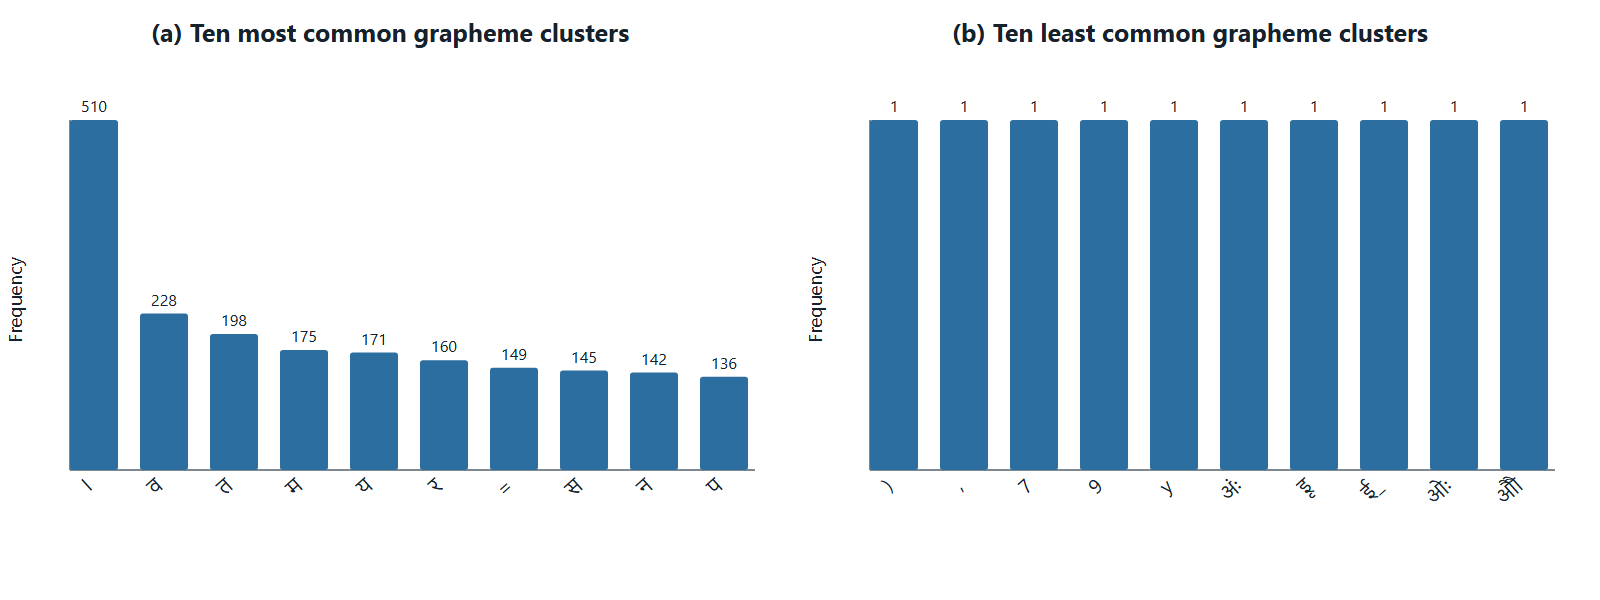
\includegraphics[width=\textwidth]{grapheme_frequency_figure.png}
\caption{Frequency of atomic grapheme clusters across all manuscripts. The \texttt{circle\_new} manuscript contains 25 active manual circular text-line orientation annotations.}
\label{fig:grapheme-frequency}
\end{figure*}
